\documentclass[12pt, letterpaper]{article}

\usepackage[utf8]{inputenc}
\usepackage{hyperref}
\usepackage{tikz}
\usepackage{minted}
\usepackage{amsmath}
\usepackage[a4paper, portrait, margin=1in]{geometry}
\usepackage{xcolor}
\usepackage{titlesec}
\usepackage{mdframed}
\usepackage{listings}

\lstset{
basicstyle=\small\ttfamily,
columns=flexible,
breaklines=true
}

\setlength{\parindent}{0em}
\setlength{\parskip}{1em}

\definecolor{smublue}{HTML}{151C55}
\definecolor{smugold}{HTML}{8A704C}
\definecolor{bg}{HTML}{C7CBF3}

\titleformat{\section}
{\color{smublue}\normalfont\Large\bfseries}
{\color{smublue}\thesection}{1em}{}

\titleformat{\subsection}
{\color{smugold}\normalfont\Large\bfseries}
{\color{smugold}\thesubsection}{1em}{}

\renewcommand{\thesection}{Question \arabic{section}}
\renewcommand{\thesubsection}{\arabic{section}\alph{subsection})}
\renewcommand{\thesubsubsection}{\roman{subsubsection})}
\renewcommand{\thefigure}{\arabic{figure}}

\title{CS601 - Introduction to Artificial Intelligence\\Assignment 1}
\author{Ian CHONG Wei Ming
\\\href{mailto:ian.chong.2020@mitb.smu.edu.sg}{ian.chong.2020@mitb.smu.edu.sg}
\\+65-9680-8118}
\date{\today}

\begin{document}
\maketitle

\section{Directed Bayesian Network}

Given the following Bayesian network:

\begin{center}
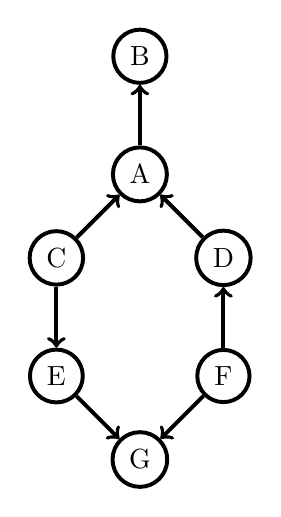
\begin{tikzpicture}[node distance={15mm},main/.style={draw,circle}]
\node[main,line width = 0.5mm] (1){B};
\node[main,line width = 0.5mm] (2) [below of=1] {A};
\node[main,line width = 0.5mm] (3) [below left of=2] {C};
\node[main,line width = 0.5mm] (4) [below right of=2] {D};
\node[main,line width = 0.5mm] (5) [below of=3] {E};
\node[main,line width = 0.5mm] (6) [below of=4] {F};
\node[main,line width = 0.5mm] (7) [below left of=6] {G};

\draw[->,line width = 0.5mm] (2) -- (1);
\draw[->,line width = 0.5mm] (3) -- (2);
\draw[->,line width = 0.5mm] (4) -- (2);
\draw[->,line width = 0.5mm] (3) -- (5);
\draw[->,line width = 0.5mm] (6) -- (4);
\draw[->,line width = 0.5mm] (5) -- (7);
\draw[->,line width = 0.5mm] (6) -- (7);
\end{tikzpicture}
\end{center}

The truth of the following statements are as follows:

\subsection{\(C\bot F\mid \{E,G\}\)}
\textbf{TRUE}. There exist two trails between C and F:

\[Trail 1: C \rightarrow \textbf{\underline{E}} \rightarrow \textbf{\underline{G}} \leftarrow F\]
\[Trail 2: C \rightarrow A \leftarrow D \leftarrow F\]

\textbf{Trail 1} is \textit{blocked}, since E and G are observed, and E blocks the trail from C to F, even if G is a collider and is \textit{observed}. 
\textbf{Trail 2} is \textit{blocked}, since E and G are observed, and A and its descendants (B) are not observed, and the two  arrows from C and F lead into A, which is a \textit{collider}. 

Since both trails between C and F are \textit{blocked}, C is \emph{d-separated} from F, and C and F are therefore \textit{conditionally independent} of each other.

\subsection{\(C\bot F\mid \{D,G\}\)}
\textbf{FALSE}. There exist two paths between C and F:

\[Trail 1: C \rightarrow E \rightarrow \textbf{\underline{G}} \leftarrow F\]
\[Trail 2: C \rightarrow A \leftarrow \textbf{\underline{D}} \leftarrow F\]

\textbf{Trail 1} is \textit{active}, since D and G are observed, and C leads into G via E, and F also leads into G, giving rise to the \textit{common effect}. 
\textbf{Path 2} is \textit{blocked}, since D and G are observed, and A and its descendants (B) are not observed, and the two path arrows from C and F lead into A, which is a \textit{collider}.

Since \emph{not all} paths between C and F are \textit{blocked}, C and F are therefore \textit{dependent} on each other.

\subsection{\(E\bot D\mid B\)}
\textbf{FALSE}. There are two trails between nodes E and D:

\[Trail 1: E \leftarrow C \rightarrow A \leftarrow D\]
\[Trail 2: E \rightarrow G \leftarrow F \rightarrow D\]

Trail 1 is \textit{active} since B is observed and is a descendant of A which gives to the \textit{common effect}.

Trail 2 is \textit{blocked} since G exists on the trail which is a \textit{collider}. 

Since there is one \textit{active} trail, E is not \textit{d separated} from D and E is \textit{dependent} on D.

\subsection{\(E\bot D\mid \{\}\)}
\textbf{TRUE}. There are two trails between nodes E and D:

\[Trail 1: E \leftarrow C \rightarrow A \leftarrow D\]
\[Trail 2: E \rightarrow G \leftarrow F \rightarrow D\]

There are no observed nodes, and both trails are blocked by \textit{colliders}. 
\textbf{Trail 1} is \textit{blocked} by A, and \textbf{Trail 2} is blocked by G. Hence, E is \textit{d-separated} from D, and they are therefore \textit{independent} of each other.

\subsection{\(A\bot F\mid \{C,D\}\)}
\textbf{TRUE}. There are two trails between nodes A and F:

\[Trail 1: A \leftarrow \textbf{\underline{D}} \rightarrow F\]
\[Trail 2: A \leftarrow \textbf{\underline{C}} \rightarrow E \rightarrow G \leftarrow F\]

C and D are observed, and D lies on \textbf{Trail 1}, \textit{blocking} the trail from F to A, while C lies on \textbf{Trail 2}, which \textit{blocks} the trail from A to F. A and F are therefore \textit{d-separated} and conditionally independent of one another.

\clearpage

\section{Box with three different dices}

\subsection{Network Diagram and Random Variable Definitions}

The Bayesian Network representing the dice and outcomes is as follows:\par

\begin{center}
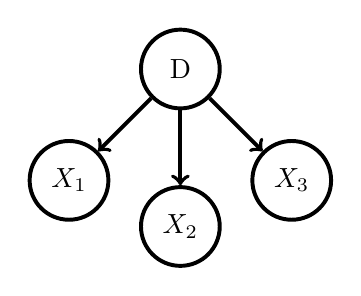
\begin{tikzpicture}[node distance={20mm},main/.style={draw,circle}]
\node[main,line width = 0.5mm,minimum size=1cm] (1){D};
\node[main,line width = 0.5mm,minimum size=1cm] (2) [below left of=1] {$X_1$};
\node[main,line width = 0.5mm,minimum size=1cm] (3) [below of=1] {$X_2$};
\node[main,line width = 0.5mm,minimum size=1cm] (4) [below right of=1] {$X_3$};

\draw[->,line width = 0.5mm] (1) -- (2);
\draw[->,line width = 0.5mm] (1) -- (3);
\draw[->,line width = 0.5mm] (1) -- (4);

\end{tikzpicture}
\end{center}

The variables $X_1$, $X_2$ and $X_3$ are all \textit{independent} of one another since the expected outcome of a dice throw is dependent only on the characteristics of the dice selected. It does not matter how many times you throw the dice.

The interpretation of the random variables are as follows:

\begin{tabular}{lll}
\textbf{RV}   & \textbf{Domain}             & \textbf{Interpretation}                             \\
D    & \{D\textsubscript{1},D\textsubscript{2},D\textsubscript{3}\} & Choice of dice between D\textsubscript{1}, D\textsubscript{2} and D\textsubscript{3} \\
X\textsubscript{1} & \{1,2,3,4\}        & The outcome of the first throw             \\
X\textsubscript{2} & \{1,2,3,4\}        & The outcome of the second throw            \\
X\textsubscript{3} & \{1,2,3,4\}        & The outcome of the third throw            
\end{tabular}

\subsection{CPT by random variable}

\subsubsection{$P(D)$}

\begin{tabular}{llll}
D=1         & D=2           & D=3           & \textbf{rowSum} \\
\hline
$\frac{1}{3}$ & $\frac{1}{3}$   & $\frac{1}{3}$   & \textbf{1}
\end{tabular}

\subsubsection{$P(X_1|D)$}
\begin{tabular}{l|llll|l}
    & $X_1$=1       & $X_1$=2       & $X_1$=3       & $X_1$=4       & \textbf{colSum} \\
\hline
D=1 & $\frac{1}{4}$   & $\frac{1}{4}$   & $\frac{1}{4}$   & $\frac{1}{4}$   & \textbf{1}  \\
D=2 & $\frac{1}{2}$   & $\frac{1}{6}$   & $\frac{1}{6}$   & $\frac{1}{6}$   & \textbf{1}  \\
D=3 & $\frac{1}{6}$   & $\frac{1}{2}$   & $\frac{1}{6}$   & $\frac{1}{6}$   & \textbf{1}  \\
\end{tabular}

\subsubsection{P($X_2|D$)}
\begin{tabular}{l|llll|l}
    & $X_2$=1       & $X_2$=2       & $X_2$=3       & $X_2$=4       & \textbf{colSum} \\
\hline
D=1 & $\frac{1}{4}$   & $\frac{1}{4}$   & $\frac{1}{4}$   & $\frac{1}{4}$   & $\textbf{1}$  \\
D=2 & $\frac{1}{2}$   & $\frac{1}{6}$   & $\frac{1}{6}$   & $\frac{1}{6}$   & $\textbf{1}$  \\
D=3 & $\frac{1}{6}$   & $\frac{1}{2}$   & $\frac{1}{6}$   & $\frac{1}{6}$   & $\textbf{1}$  \\
\end{tabular}

\subsubsection{P($X_3|D$)}
\begin{tabular}{l|llll|l}
    & $X_3$=1       & $X_3$=2       & $X_3$=3       & $X_3$=4       & \textbf{colSum} \\
\hline
D=1 & $\frac{1}{4}$   & $\frac{1}{4}$   & $\frac{1}{4}$   & $\frac{1}{4}$   & $\textbf{1}$  \\
D=2 & $\frac{1}{2}$   & $\frac{1}{6}$   & $\frac{1}{6}$   & $\frac{1}{6}$   & $\textbf{1}$  \\
D=3 & $\frac{1}{6}$   & $\frac{1}{2}$   & $\frac{1}{6}$   & $\frac{1}{6}$   & $\textbf{1}$  \\
\end{tabular}

\subsection{$P(D|X_1=1,X_2=3,X_3=2)$}

For a dice $d$, the probability that it gets picked given $X_1=1$, $X_2=3$ and $X_3=2$ is given by the following

\begin{align*}
&P(D=d|X_1=1,X_2=3,X_3=2) = \frac{P(D=d,X_1=1,X_2=3,X_3=2)}{P(X_1=1,X_2=3,X_3=2)}\\ 
                            &= \frac{P(D=d,X_1=1,X_2=3,X_3=2)}{\sum_{d\in D}{P(D=d)P(X_1=1|D=d)P(X_2=3|D=d)P(X_3=2|D=d)}}
\end{align*}

We can can calculate the denominator for the above as follows

\begin{align*}
P(X_1=1,X_2=3,X_3=2)    &= \sum_{d\in D}{P(D=d)P(X_1=1|D=d)P(X_2=3|D=d)P(X_3=2|D=d)}\\
                        &= \bigg( \frac{1}{3}\cdot\frac{1}{4}\cdot\frac{1}{4}\cdot\frac{1}{4}\bigg) + \bigg(\frac{1}{3}\cdot\frac{1}{2}\cdot\frac{1}{6}\cdot\frac{1}{6}\bigg)+\bigg(\frac{1}{3}\cdot\frac{1}{6}\cdot\frac{1}{6}\cdot\frac{1}{2}\bigg)\\
                        &= 0.0052083+0.0046296+0.0046296\\
                        &= 0.014468
\end{align*}

\begin{align*}
P(D=1|X_1=1,X_2=3,X_3=2)    &= \frac{0.0052083}{0.014468}\\ 
                            &= \underline{\textbf{0.36}}\\                            
\end{align*}

\begin{align*} 
P(D=2|X_1=1,X_2=3,X_3=2)    &= \frac{0.0046296}{0.014468}\\ 
                            &= \textbf{\underline{0.32}}
\end{align*}

\begin{align*} 
P(D=3|X_1=1,X_2=3,X_3=2)    &= \frac{0.0046296}{0.014468}\\ 
                            &= \textbf{\underline{0.32}}
\end{align*}

Since the highest joint probability of the outcomes occurs when D=1, it \textit{most likely} that \textbf{$D_1$} was picked from the box.

\clearpage

\section{Constructing a BayesNet with \texttt{pgmpy}}

The following random variables all have outcomes $\in \{0,1\}$

\begin{tabular}{ll}
\textbf{Description}   & \textbf{Random Variable}\\
\hline
Yellow fingers&$Y\in \{0,1\}$\\
Smoking&$S\in \{0,1\}$\\
Cancer&$C\in \{0,1\}$\\
Weakness&$W\in \{0,1\}$\\
Radiation&$R\in \{0,1\}$\\
Solar flare&$F\in \{0,1\}$\\
Using microwave&$M\in \{0,1\}$\\
\end{tabular}

\subsection{\texttt{pgmpy} code}

The following code constructs the BayesNet

\begin{mdframed}[backgroundcolor=bg]
\begin{minted}[fontsize=\footnotesize,breaklines]{python}
from pgmpy.models import BayesianModel
from pgmpy.factors.discrete import TabularCPD
# We first create a model which containts edges of the graph
model = BayesianModel([('S','Y'),
                       ('S','W'),
                       ('S','C'),
                       ('F','R'),
                       ('M','R'),
                       ('R','C')])

# Enter conditional probability distribution for each variable

# Prior probability for smoking P(S)
cpd_S = TabularCPD(variable='S', variable_card=2, values=[[0.85],[0.15]])

# Prior probability for solar flare P(F)
cpd_F = TabularCPD(variable='F', variable_card=2, values=[[0.99],[0.01]])

# Prior probability for micro wave P(M)
cpd_M = TabularCPD(variable='M', variable_card=2, values=[[0.05],[0.95]])

# Conditional probability for weakness W or P(W|S)
cpd_W = TabularCPD(variable='W',variable_card=2,
                    values = [[0.8,0.1],[0.2,0.9]],
                    evidence = ['S'],
                    evidence_card=[2])

# Conditional probability for radiation R or P(R|F,M)
cpd_R = TabularCPD(variable='R', variable_card=2,
                    values = [[0.9, 0.8, 0.8, 0.1],[0.1, 0.2, 0.2, 0.9]],
                    evidence = ['F','M'],
                    evidence_card=[2,2])

# Conditional probability for cancer C or P(C|S,R)
cpd_C = TabularCPD(variable='C', variable_card=2, 
                    values = [[0.9, 0.4, 0.7, 0.1],[0.1, 0.6, 0.3, 0.9]],                             
                    evidence = ['S','R'],
                    evidence_card=[2,2])

# Conditional probability for yellow fingers Y or P(Y|S)
cpd_Y = TabularCPD(variable='Y',variable_card=2,
                    values = [[0.89,0.2],[0.11,0.8]],
                    evidence = ['S'], 
                    evidence_card=[2])

# Add CPDs to the model
model.add_cpds(cpd_S, cpd_F, cpd_M, cpd_W, cpd_R, cpd_C, cpd_Y)

cpds = model.get_cpds()
for cpd in cpds:
    evidence = ",".join(cpd.variables[1:])
    if evidence:
        print(f"P({cpd.variables[0]}|{evidence})")
    else:
        print(f"P({cpd.variables[0]})")
    print(cpd)
\end{minted}
\end{mdframed}

Print of the results as follows
\begin{mdframed}[backgroundcolor=bg]
\begin{lstlisting}
P(S)
+------+------+
| S(0) | 0.85 |
+------+------+
| S(1) | 0.15 |
+------+------+
P(F)
+------+------+
| F(0) | 0.99 |
+------+------+
| F(1) | 0.01 |
+------+------+
P(M)
+------+------+
| M(0) | 0.05 |
+------+------+
| M(1) | 0.95 |
+------+------+
P(W|S)
+------+------+------+
| S    | S(0) | S(1) |
+------+------+------+
| W(0) | 0.8  | 0.1  |
+------+------+------+
| W(1) | 0.2  | 0.9  |
+------+------+------+
P(R|F,M)
+------+------+------+------+------+
| F    | F(0) | F(0) | F(1) | F(1) |
+------+------+------+------+------+
| M    | M(0) | M(1) | M(0) | M(1) |
+------+------+------+------+------+
| R(0) | 0.9  | 0.8  | 0.8  | 0.1  |
+------+------+------+------+------+
| R(1) | 0.1  | 0.2  | 0.2  | 0.9  |
+------+------+------+------+------+
P(C|S,R)
+------+------+------+------+------+
| S    | S(0) | S(0) | S(1) | S(1) |
+------+------+------+------+------+
| R    | R(0) | R(1) | R(0) | R(1) |
+------+------+------+------+------+
| C(0) | 0.9  | 0.4  | 0.7  | 0.1  |
+------+------+------+------+------+
| C(1) | 0.1  | 0.6  | 0.3  | 0.9  |
+------+------+------+------+------+
P(Y|S)
+------+------+------+
| S    | S(0) | S(1) |
+------+------+------+
| Y(0) | 0.89 | 0.2  |
+------+------+------+
| Y(1) | 0.11 | 0.8  |
+------+------+------+
\end{lstlisting}    
\end{mdframed}

\subsection{Reponses}
\subsubsection{Draw the Bayesian Network}

The random variables defined earlier are arranged in a Bayesian Network as follows:
\begin{center}
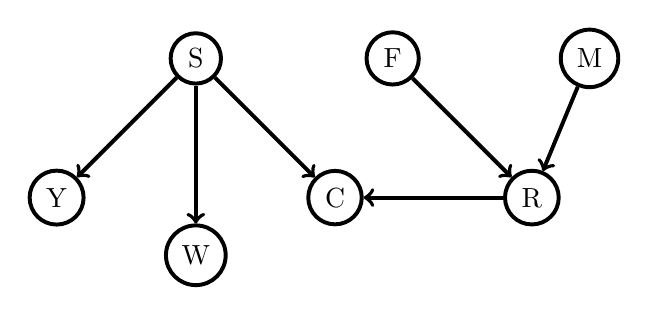
\begin{tikzpicture}[node distance={25mm},main/.style={draw,circle}]
\node[main,line width = 0.5mm] (1){S};
\node[main,line width = 0.5mm] (2) [right of=1] {F};
\node[main,line width = 0.5mm] (3) [right of=2] {M};
\node[main,line width = 0.5mm] (4) [below left of=1] {Y};
\node[main,line width = 0.5mm] (5) [below of=1] {W};
\node[main,line width = 0.5mm] (6) [below right of=1] {C};
\node[main,line width = 0.5mm] (7) [below right of=2] {R};

\draw[->,line width =0.5mm] (1) -- (4);
\draw[->,line width =0.5mm] (1) -- (5);
\draw[->,line width =0.5mm] (1) -- (6);
\draw[->,line width =0.5mm] (2) -- (7);
\draw[->,line width =0.5mm] (3) -- (7);
\draw[->,line width =0.5mm] (7) -- (6);
    
\end{tikzpicture}    
\end{center}

\subsubsection{Probability of cancer given weakness=1}

Running the following code in \texttt{python}:

\begin{mdframed}[backgroundcolor=bg]
\begin{minted}[fontsize=\footnotesize,breaklines]{python}
from pgmpy.inference import VariableElimination
infer = VariableElimination(model)
phi_query = infer.query(['C'], evidence={'W':1}, joint = False)
factor = phi_query['C']
print('Probability C|W')
print(factor)
\end{minted}
\end{mdframed}

Gives the following output:

\begin{mdframed}[backgroundcolor=bg]
\begin{lstlisting}
Probability C|W
+------+----------+
| C    |   phi(C) |
+======+==========+
| C(0) |   0.7017 |
+------+----------+
| C(1) |   0.2983 |
+------+----------+
\end{lstlisting}
\end{mdframed}

$P(C=1|W=1)=\underline{\textbf{0.2983}}$

\subsubsection{Probability of smoking given cancer=1}

Running the following:

\begin{mdframed}[backgroundcolor=bg]
\begin{minted}[fontsize=\footnotesize,breaklines]{python} 
phi_query = infer.query(['S'], evidence={'C':1}, joint = False)
factor = phi_query['S']
print('Probability S|C')
print(factor)
\end{minted}
\end{mdframed}

Gives the following output:

\begin{mdframed}[backgroundcolor=bg]
\begin{lstlisting}
+------+----------+
| S    |   phi(S) |
+======+==========+
| S(0) |   0.7300 |
+------+----------+
| S(1) |   0.2700 |
+------+----------+
\end{lstlisting}
\end{mdframed}

$P(S=1|C=1)=\underline{\textbf{0.2700}}$

\subsubsection{Smoking and Radiation independent given cancer?}
In order for S and R to be independent given C, we need to prove

\[P(S=1,R=1|C=1)=P(S=1|C=1)\times P(R=1|C=1)\]

To find $P(S-1,R=1|C=1)$, we run the following Python code:

\begin{mdframed}[backgroundcolor=bg]
\begin{minted}[fontsize=\footnotesize,breaklines]{python}
phi_query = infer.query(['S','R'],evidence={'C':1})
print(phi_query)
\end{minted}
\end{mdframed}

We achieve the following results:

\begin{mdframed}[backgroundcolor=bg]
\begin{lstlisting}
+------+------+------------+
| S    | R    |   phi(S,R) |
+======+======+============+
| S(0) | R(0) |     0.2901 |
+------+------+------------+
| S(0) | R(1) |     0.4398 |
+------+------+------------+
| S(1) | R(0) |     0.1536 |
+------+------+------------+
| S(1) | R(1) |     0.1164 |
+------+------+------------+
\end{lstlisting}
\end{mdframed}

We have $P(S=1,R=1|C=1)=\textbf{\underline{0.1164}}$

Similarly, we achieve $P(S=1|C=1)=\textbf{0.27}$ and $P(R=1|C=1)=\textbf{0.5563}$. Multiplying the two probabilities we get

\[0.27\times 0.5563=0.150201\neq P(S=1,R=1|C=1)\]

Hence, S and R are not \textit{conditionally independent}

Alternatively, there exists only one path between S and R:

$S\rightarrow C\leftarrow R$

Since C is observed, the path is \textit{active} and S and R are \textit{dependent} given C.

\subsubsection{Probability of cancer without microwave}

Running the following Python code:

\begin{mdframed}[backgroundcolor=bg]
\begin{minted}[fontsize=\footnotesize,breaklines]{python}
phi_query = infer.query(['C'],evidence={"M":0})
print(phi_query)
\end{minted}
\end{mdframed}

We get the output

\begin{mdframed}[backgroundcolor=bg]
\begin{lstlisting}
+------+----------+
| C    |   phi(C) |
+======+==========+
| C(0) |   0.8180 |
+------+----------+
| C(1) |   0.1820 |
+------+----------+
\end{lstlisting}
\end{mdframed}

$P(C=1|M=0)=\textbf{\underline{0.1820}}$

\clearpage

\section{Fashion MNIST dataset}

{\large Preamble}

\begin{mdframed}[backgroundcolor=bg]
\begin{minted}[fontsize=\footnotesize,breaklines]{python}
import tensorflow as tf
from tensorflow.keras.models import Sequential
from tensorflow.keras import layers
from tensorflow.keras.utils import to_categorical
from tensorflow.keras.optimizers import Adagrad
from tensorflow.keras.losses import CategoricalCrossentropy
from tensorflow.keras.metrics import CategoricalAccuracy
from tensorflow.keras.callbacks import ReduceLROnPlateau, ModelCheckpoint

from sklearn.metrics import confusion_matrix, classification_report, accuracy_score
import numpy as np
from matplotlib import pyplot as plt
import seaborn as sns

directory = 'fashion_MNIST_checkpoint'
epochs = 30
optimizer = Adagrad(learning_rate=0.005,initial_accumulator_value=0.05,epsilon=1e-6)

model_checkpoint_callback = ModelCheckpoint(
    filepath=directory,
    save_weights_only=True,
    monitor='categorical_cross_entropy',
    mode='max',
    save_best_only=True)
reduce_lr = ReduceLROnPlateau(
    monitor='loss',
    factor = 0.2,
    patience = 5,
    min_lr = 0.0001
)
\end{minted}
\end{mdframed}

{\large Download Fashion MNIST and Preprocessing}

Fulfils 4a

\begin{mdframed}[backgroundcolor=bg]
\begin{minted}[fontsize=\footnotesize,breaklines]{python}
fashion_mnist = tf.keras.datasets.fashion_mnist
(train_images, train_labels), (test_images, test_labels) = fashion_mnist.load_data()
train_images = train_images/255.0
test_images = test_images/255.0
print([train_images.shape,test_images.shape,train_labels.shape,test_labels.shape])
size = 28
train_count = len(train_images)
test_count = len(test_images)
input_shape = (size,size,1)
train_images_shaped = train_images.reshape(train_count,size,size,1)
test_images_shaped = test_images.reshape(test_count,size,size,1)
train_labels_shaped = to_categorical(train_labels)
test_labels_shaped = to_categorical(test_labels)
\end{minted}
\end{mdframed}

{\large Neural Network Architecture}

Fulfils 4b and 4c
\begin{mdframed}[backgroundcolor=bg]
\begin{minted}[fontsize=\footnotesize,breaklines]{python}
model = Sequential()
model.add(layers.Dense(64,activation='relu'))
model.add(layers.Dropout(0.2))
model.add(layers.Dense(256, activation='relu'))
model.add(layers.Dropout(0.2))
model.add(layers.Dense(128, activation='relu'))
model.add(layers.Dropout(0.1))
model.add(layers.Flatten())
model.add(layers.Dense(10,activation='softmax'))
\end{minted}
\end{mdframed}

The activation function used in the last layer was \texttt{softmax} 
because this is a multilabel classification exercise

{\large Compiling and Training the Network}

Fulfils 4d

\begin{mdframed}[backgroundcolor=bg]
\begin{minted}[fontsize=\footnotesize,breaklines]{python}
model.compile(
    optimizer=optimizer,
    loss="categorical_crossentropy",
    metrics=[CategoricalCrossentropy(),CategoricalAccuracy()])

history = model.fit(
    train_images_shaped,
    train_labels_shaped,
    epochs=epochs,
    callbacks=[model_checkpoint_callback,reduce_lr])
\end{minted}
\end{mdframed}

The loss function chosen was \texttt{categorical\_crossentropy} because the labels were one hot encoded which changed the shape of the output.

Output as follows:

\begin{mdframed}[backgroundcolor=bg]
\begin{lstlisting}
Epoch 1/30
1875/1875 [==============================] - 14s 7ms/step - loss: 0.7719 - categorical_crossentropy: 0.7719 - categorical_accuracy: 0.7425
WARNING:tensorflow:Can save best model only with categorical_cross_entropy available, skipping.
Epoch 2/30
1875/1875 [==============================] - 13s 7ms/step - loss: 0.4390 - categorical_crossentropy: 0.4390 - categorical_accuracy: 0.8456
WARNING:tensorflow:Can save best model only with categorical_cross_entropy available, skipping.
Epoch 3/30
1875/1875 [==============================] - 13s 7ms/step - loss: 0.4098 - categorical_crossentropy: 0.4098 - categorical_accuracy: 0.8554
WARNING:tensorflow:Can save best model only with categorical_cross_entropy available, skipping.
Epoch 4/30
1875/1875 [==============================] - 13s 7ms/step - loss: 0.3900 - categorical_crossentropy: 0.3900 - categorical_accuracy: 0.8612
WARNING:tensorflow:Can save best model only with categorical_cross_entropy available, skipping.
Epoch 5/30
1875/1875 [==============================] - 13s 7ms/step - loss: 0.3737 - categorical_crossentropy: 0.3737 - categorical_accuracy: 0.8660
WARNING:tensorflow:Can save best model only with categorical_cross_entropy available, skipping.
\end{lstlisting}
\end{mdframed}

\dots
Skipping for brevity's sake
\dots

\begin{mdframed}[backgroundcolor=bg]
\begin{lstlisting}
Epoch 26/30
1875/1875 [==============================] - 13s 7ms/step - loss: 0.3080 - categorical_crossentropy: 0.3080 - categorical_accuracy: 0.8887
WARNING:tensorflow:Can save best model only with categorical_cross_entropy available, skipping.
Epoch 27/30
1875/1875 [==============================] - 13s 7ms/step - loss: 0.2973 - categorical_crossentropy: 0.2973 - categorical_accuracy: 0.8910
WARNING:tensorflow:Can save best model only with categorical_cross_entropy available, skipping.
Epoch 28/30
1875/1875 [==============================] - 13s 7ms/step - loss: 0.2967 - categorical_crossentropy: 0.2967 - categorical_accuracy: 0.8908
WARNING:tensorflow:Can save best model only with categorical_cross_entropy available, skipping.
Epoch 29/30
1875/1875 [==============================] - 13s 7ms/step - loss: 0.2994 - categorical_crossentropy: 0.2994 - categorical_accuracy: 0.8914
WARNING:tensorflow:Can save best model only with categorical_cross_entropy available, skipping.
Epoch 30/30
1875/1875 [==============================] - 13s 7ms/step - loss: 0.2958 - categorical_crossentropy: 0.2958 - categorical_accuracy: 0.8927
WARNING:tensorflow:Can save best model only with categorical_cross_entropy available, skipping.
\end{lstlisting}
\end{mdframed}

{\large 1) Confusion Matrix}

The code to generate the confusion matrix in Figure~\ref{fig:fashionmnist-1} is as follows:

\begin{mdframed}[backgroundcolor=bg]
\begin{minted}[fontsize=\footnotesize,breaklines]{python}
test_labels_predicted = np.argmax(model.predict(test_images_shaped), axis=1)
cm = confusion_matrix(test_labels, test_labels_predicted)
plt.figure(dpi=100,figsize=(6,6))
ax=plt.gca()
sns.heatmap(cm, annot=True, fmt='.0f', cmap='Blues',ax=ax)
plt.title("Fashion MNIST Confusion Matrix")
plt.ylabel("Actual")
plt.xlabel("Predicted")
\end{minted}
\end{mdframed}

\begin{figure}
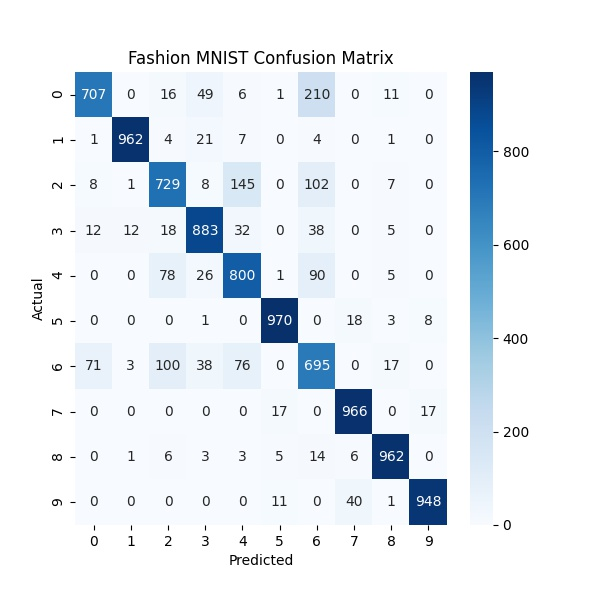
\includegraphics[width=\linewidth]{colab_fashion_mnist_cm.jpeg}
\caption{\textit{Fashion MNIST} confusion matrix}
\label{fig:fashionmnist-1}
\end{figure}

{\large 2) Loss Function}

The loss function was \texttt{categorical\_crossentropy}. Plot code to generate the result in Figure~\ref{fig:fashionmnist-2} is as follows:

\begin{mdframed}[backgroundcolor=bg]
\begin{minted}[fontsize=\footnotesize,breaklines]{python}
import pandas as pd
training_data = pd.DataFrame(history.history)
plt.figure(dpi=100)
plt.title("Fashion MNIST Training Data")
plt.xlabel("Epoch")
ax = plt.gca()
training_data['categorical_crossentropy'].plot(ax=ax)
training_data['categorical_accuracy'].plot(ax=ax)
plt.legend()
\end{minted}
\end{mdframed}

\begin{figure}
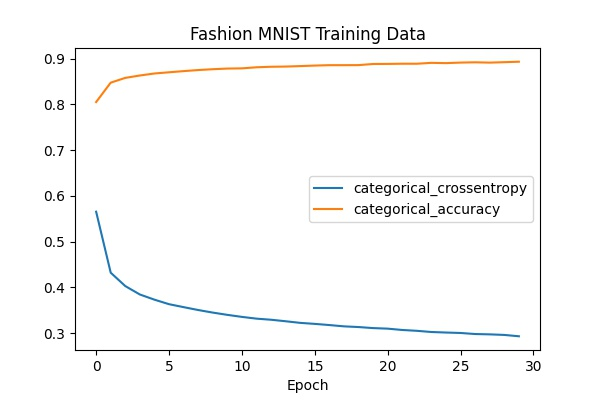
\includegraphics[width=\linewidth]{colab_fashion_mnist_training.jpeg}
\caption{\textit{Fashion MNIST} loss over time}
\label{fig:fashionmnist-2}
\end{figure}

{\large 3) Accuracy}

Running the following line gives us accuracy on testing data of \underline{\textbf{86\%}}
\begin{verbatim}
model.evaluate(test_images_shaped,test_labels_shaped)
\end{verbatim}

\clearpage

\section{MobileNetV2 Transfer Learning}

\subsection{\texttt{python} code}

{\large Preamble}

\begin{mdframed}[backgroundcolor=bg]
\begin{minted}[fontsize=\footnotesize,breaklines]{python}
import tensorflow as tf
from tensorflow.keras import Model
from tensorflow.keras.layers import Input, MaxPool2D, Dropout,Dense, Conv2D, Flatten
from tensorflow.keras.callbacks import ReduceLROnPlateau
from tensorflow.keras import Sequential
from tensorflow.keras.applications import MobileNetV2
from tensorflow.keras.datasets import cifar10
from tensorflow.keras.preprocessing.image import ImageDataGenerator
from tensorflow.keras.optimizers import RMSprop
from tensorflow.keras.metrics import SparseCategoricalAccuracy, SparseCategoricalCrossentropy

from sklearn.metrics import accuracy_score, confusion_matrix
import seaborn as sns

import cv2

import sys
import numpy as np
import csv
import math
import os

from matplotlib import pyplot as plt
\end{minted}
\end{mdframed}

{\large Key Notebook Parameters}

I define key parameters of the notebook early on to facilitate transparency.

\begin{tabular}{ll}
\hline
\textbf{Input} & \textbf{Description}\\
\hline
\texttt{use\_sample}                &Trigger sampling of data to facilitate faster prototyping\\
\texttt{sample\_probability}        &Chance that a row is selected to be a sample\\
\texttt{use\_datagen}               &Trigger \texttt{ImageDataGenerator} usage\\
\texttt{force\_restart}             &Ignore existing model and train new model from scratch\\
\texttt{epochs}                     &Number of times to train over the dataset\\
\texttt{metrics}                    &Metric classes to be included in the \texttt{.fit\(\)} phase\\
\texttt{final\_layer\_activation}   &Activation function to use in the last layer\\
\texttt{optimizer}                  &Optimizer for model compilation\\
\texttt{loss}                       &Loss function for model compilation\\
\texttt{reduce\_lr}                 &\texttt{LRReduceOnPlateau} callback to reduce learning rate \\
&after stagnation\\
\texttt{directory}                  &model saved directory
\end{tabular}

The classes for the dataset are the following:

\begin{tabular}{ll}
\hline
\textbf{Class No.} & \textbf{Description}\\
\hline
0&airplane\\
1&automobile\\
2&bird\\
3&cat\\
4&deer\\
5&dog\\
6&frog\\
7&horse\\
8&ship\\
9&truck\\
\end{tabular}

The code is as follows:

\begin{mdframed}[backgroundcolor=bg]
\begin{minted}[fontsize=\footnotesize,breaklines]{python}
use_sample = False
sample_probability = 0.05
use_datagen = False
force_restart = False

epochs = 10
metrics = [SparseCategoricalAccuracy("sparse_categorical_accuracy"), SparseCategoricalCrossentropy(name="sparse_categorical_cross_entropy")]

final_layer_activation = 'softmax'
optimizer = RMSprop(learning_rate=0.001)
loss = 'sparse_categorical_crossentropy'
reduce_lr = ReduceLROnPlateau(monitor='loss', factor=0.2,patience=3, min_lr=0.0005)

directory = "cs601_mobilenetv2_saved"

if not os.path.exists(directory):
    os.makedirs(directory)
    print("Directory created at [{}]!".format(directory))
else:
    "Directory [{}] exists!"
\end{minted}
\end{mdframed}

{\large Import Dataset}

\begin{mdframed}[backgroundcolor=bg]
\begin{minted}[fontsize=\footnotesize,breaklines]{python}
# Class names for different classes
class_names = ['airplane', 'automobile', 'bird', 'cat','deer','dog', 'frog', 'horse', 'ship', 'truck']

# Load training data, labels; and testing data and their true labels
(train_images, train_labels), (test_images, test_labels) = cifar10.load_data()

if use_sample:
    mask = np.random.choice([False, True], len(train_images),p=[1 - sample_probability, sample_probability])
    train_images, train_labels = train_images[mask], train_labels[mask]

# Normalize pixel values between -1 and 1
train_images = train_images / 127.5 - 1 
test_images = test_images / 127.5 - 1 

print ('Training data size:', train_images.shape, 
        'Test data size', test_images.shape)
\end{minted}
\end{mdframed}

{\large Visualize Dataset}

\begin{mdframed}[backgroundcolor=bg]
\begin{minted}[fontsize=\footnotesize,breaklines]{python}
%matplotlib inline
#Show first 25 training images below
plt.figure(figsize=(10,10))
for i in range(25):
    plt.subplot(5,5,i+1)
    plt.xticks([])
    plt.yticks([])
    plt.grid(False)
    plt.imshow(train_images[i], cmap=plt.cm.binary)
    plt.xlabel(class_names[train_labels[i][0]])
\end{minted}
\end{mdframed}

{\large Resize Images for \texttt{MobileNetV2} model}

\begin{mdframed}[backgroundcolor=bg]
\begin{minted}[fontsize=\footnotesize,breaklines]{python}
# Upsize images to 96x96 for use with MobileNetV2
minSize = 96 #minimum size requried for mobileNetV2
class_num = len(class_names)
image_num_train = len(train_images)
image_num_test = len(test_images)

# You may use cv2 package. Look for function:
resized_train_images = np.zeros((image_num_train, minSize, minSize, 3), 
                                    dtype=np.float32)

resized_test_images = np.zeros((image_num_test, minSize, minSize, 3), 
                                    dtype=np.float32)

for index, image in enumerate(train_images):
    resized_train_images[index]=cv2.resize(image,dsize=(minSize, minSize), interpolation=cv2.INTER_AREA)

for index, image in enumerate(test_images):
    cv2.resize(i, dsize=(minSize, minSize),interpolation=cv2.INTER_AREA)
    resized_test_images[index]=cv2.resize(image,dsize=(minSize, minSize), interpolation=cv2.INTER_AREA)
\end{minted}
\end{mdframed}

{\large Download \texttt{MobileNetV2} model}

The code here fulfils part 5a and 5b and 5c.

\begin{mdframed}[backgroundcolor=bg]
\begin{minted}[fontsize=\footnotesize,breaklines]{python}
def make_model():
    """Create new MobileNetV2 model with frozen layers
    """
    # Initiate MobileNetV2 and freeze layers
    base_model = MobileNetV2(weights='imagenet', include_top=False, input_shape=input_shape)
    base_model.trainable = False

    model = Sequential()
    model.add(base_model)
    model.add(Conv2D(filters=16, kernel_size=(5, 5),strides=(2,2), padding='same', activation='relu'))
    model.add(Conv2D(filters=16, kernel_size=(5, 5),strides=(2,2), padding='same', activation='relu'))
    model.add(MaxPool2D(pool_size=(4, 4),strides=(2,2), padding='same'))
    model.add(Dropout(0.1))
    model.add(Conv2D(filters=32, kernel_size=(4, 4), padding='same', activation='relu'))
    model.add(Conv2D(filters=32, kernel_size=(4, 4), padding='same', activation='relu'))
    model.add(MaxPool2D(pool_size=(3, 3), padding='same'))
    model.add(Dropout(0.1))
    model.add(Conv2D(filters=64, kernel_size=(3, 3), padding='same', activation='relu'))
    model.add(Conv2D(filters=64, kernel_size=(3, 3), padding='same', activation='relu'))
    model.add(MaxPool2D(pool_size=(2, 2), padding='same'))
    model.add(Dropout(0.1))
    model.add(Dense(128, activation='relu'))
    model.add(Flatten())
    model.add(Dense(class_num, activation=final_layer_activation))
    return model

# Train new model if force_restart is True
# Else, if existing model detected, load it for further training
# Finally, create new model if all else fails

if force_restart:
    print("Force restart enabled")
    model = make_model()
    print("Created new model!")
else:
    try:
        print("Loading existing model from [{}]".format(directory))
        model = tf.keras.models.load_model(directory)
        print("Loaded model successfully!")
    except:
        model = make_model()
        print("Created new model!")

\end{minted}
\end{mdframed}

{\large Add loss function, compile and train the model, and check accuracy on test data}

Fulfils part 5d

\begin{mdframed}[backgroundcolor=bg]
\begin{minted}[fontsize=\footnotesize,breaklines]{python}
model.compile(optimizer=optimizer,loss=loss,metrics=metrics)
model_checkpoint_callback = tf.keras.callbacks.ModelCheckpoint(
    filepath=os.path.join(directory,"checkpoints"),monitor="val_loss")
history = model.fit(
    x=resized_train_images,
    y=train_labels,
    epochs=epochs,
    callbacks=[reduce_lr,model_checkpoint_callback])
\end{minted}
\end{mdframed}


\texttt{model.summary()} returns the following:

\begin{mdframed}[backgroundcolor=bg]
\begin{lstlisting}

model.compile(optimizer=optimizer,loss=loss,metrics=metrics)
model.summary()
Model: "sequential"
_________________________________________________________________
Layer (type)                 Output Shape              Param #   
=================================================================
mobilenetv2_1.00_96 (Functio (None, 3, 3, 1280)        2257984   
_________________________________________________________________
conv2d (Conv2D)              (None, 2, 2, 16)          512016    
_________________________________________________________________
conv2d_1 (Conv2D)            (None, 1, 1, 16)          6416      
_________________________________________________________________
max_pooling2d (MaxPooling2D) (None, 1, 1, 16)          0         
_________________________________________________________________
dropout (Dropout)            (None, 1, 1, 16)          0         
_________________________________________________________________
conv2d_2 (Conv2D)            (None, 1, 1, 32)          8224      
_________________________________________________________________
conv2d_3 (Conv2D)            (None, 1, 1, 32)          16416     
_________________________________________________________________
max_pooling2d_1 (MaxPooling2 (None, 1, 1, 32)          0         
_________________________________________________________________
dropout_1 (Dropout)          (None, 1, 1, 32)          0         
_________________________________________________________________
conv2d_4 (Conv2D)            (None, 1, 1, 64)          18496     
_________________________________________________________________
conv2d_5 (Conv2D)            (None, 1, 1, 64)          36928     
_________________________________________________________________
max_pooling2d_2 (MaxPooling2 (None, 1, 1, 64)          0         
_________________________________________________________________
dropout_2 (Dropout)          (None, 1, 1, 64)          0         
_________________________________________________________________
dense (Dense)                (None, 1, 1, 128)         8320      
_________________________________________________________________
flatten (Flatten)            (None, 128)               0         
_________________________________________________________________
dense_1 (Dense)              (None, 10)                1290      
=================================================================
Total params: 2,866,090
Trainable params: 608,106
Non-trainable params: 2,257,984
_________________________________________________________________
\end{lstlisting}
\end{mdframed}

{\large Training Output}

\begin{mdframed}[backgroundcolor=bg]
\begin{lstlisting}
Epoch 1/50
1563/1563 [==============================] - 122s 76ms/step - loss: 1.4577 - sparse_categorical_accuracy: 0.4273 - sparse_categorical_cross_entropy: 1.4577
INFO:tensorflow:Assets written to: cs601_mobilenetv2_saved/checkpoints/assets
Epoch 2/50
1563/1563 [==============================] - 115s 73ms/step - loss: 0.8207 - sparse_categorical_accuracy: 0.7390 - sparse_categorical_cross_entropy: 0.8207
INFO:tensorflow:Assets written to: cs601_mobilenetv2_saved/checkpoints/assets
Epoch 3/50
1563/1563 [==============================] - 117s 75ms/step - loss: 0.6683 - sparse_categorical_accuracy: 0.7889 - sparse_categorical_cross_entropy: 0.6683
INFO:tensorflow:Assets written to: cs601_mobilenetv2_saved/checkpoints/assets
Epoch 4/50
1563/1563 [==============================] - 106s 68ms/step - loss: 0.5803 - sparse_categorical_accuracy: 0.8214 - sparse_categorical_cross_entropy: 0.5803
INFO:tensorflow:Assets written to: cs601_mobilenetv2_saved/checkpoints/assets
Epoch 5/50
1563/1563 [==============================] - 124s 79ms/step - loss: 0.5209 - sparse_categorical_accuracy: 0.8424 - sparse_categorical_cross_entropy: 0.5209
INFO:tensorflow:Assets written to: cs601_mobilenetv2_saved/checkpoints/assets
\end{lstlisting}
\end{mdframed}

\dots Leaving out the middle for brevity's sake \dots

\begin{mdframed}[backgroundcolor=bg]
\begin{lstlisting}
Epoch 46/50
1563/1563 [==============================] - 99s 64ms/step - loss: 0.2797 - sparse_categorical_accuracy: 0.9544 - sparse_categorical_cross_entropy: 0.2797
INFO:tensorflow:Assets written to: cs601_mobilenetv2_saved/checkpoints/assets
Epoch 47/50
1563/1563 [==============================] - 94s 60ms/step - loss: 0.2568 - sparse_categorical_accuracy: 0.9564 - sparse_categorical_cross_entropy: 0.2568
INFO:tensorflow:Assets written to: cs601_mobilenetv2_saved/checkpoints/assets
Epoch 48/50
1563/1563 [==============================] - 96s 61ms/step - loss: 0.2764 - sparse_categorical_accuracy: 0.9557 - sparse_categorical_cross_entropy: 0.2764
INFO:tensorflow:Assets written to: cs601_mobilenetv2_saved/checkpoints/assets
Epoch 49/50
1563/1563 [==============================] - 94s 60ms/step - loss: 0.2971 - sparse_categorical_accuracy: 0.9542 - sparse_categorical_cross_entropy: 0.2971
INFO:tensorflow:Assets written to: cs601_mobilenetv2_saved/checkpoints/assets
Epoch 50/50
1563/1563 [==============================] - 96s 61ms/step - loss: 0.3920 - sparse_categorical_accuracy: 0.9555 - sparse_categorical_cross_entropy: 0.3920
INFO:tensorflow:Assets written to: cs601_mobilenetv2_saved/checkpoints/assets
\end{lstlisting}
\end{mdframed}

\subsection{Explanation}

\subsubsection{Write how you extended the MobileNetV2 model}
\begin{itemize}
\item \textbf{How many layers you added:} I added 14 layers as the images were larger than the \texttt{Fashion MNIST} data set, and had more features to extract.
\item \textbf{What type of layers:} I used \texttt{Conv2D} and \texttt{MaxPooling2D} layers to extract features and \texttt{Dropout} layers to ensure the weights of neurons do not go to zero as well as to reduce overfitting.
\item \textbf{How many nodes per layer:} I used \underline{\textbf{128}} nodes at the last layer.
\item \textbf{Their activation function:} I used \texttt{relu} for all the hidden layers and \texttt{softmax} for the output layer.
\end{itemize}
 
\subsubsection{Plot the loss function value with respect to the epoch number on the training data. How did you decide when to terminate training?}

\begin{figure}[h!]
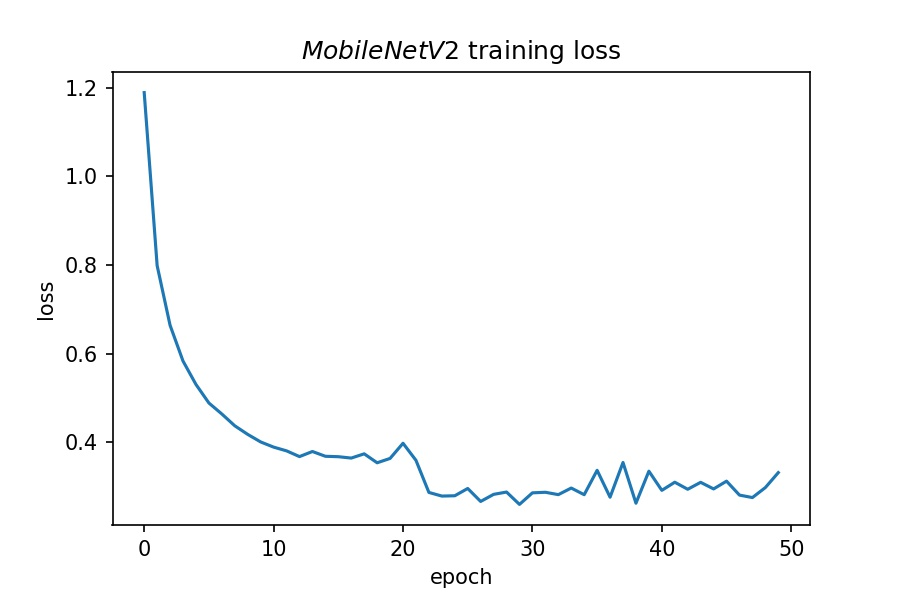
\includegraphics[width=\linewidth]{history_loss.jpeg}
\caption{\texttt{MobileNetV2} training loss}
\label{fig:mobilenetv2-1}
\end{figure}

The model was trained over 50 epochs on a Colab Pro instance. 

The loss stopped improving past the \textbf{23rd epoch} as per Figure~\ref{fig:mobilenetv2-1}.

\subsubsection{Show the accuracy of the trained classifier over the entire testing dataset.}

Training accuracy was high at over \textbf{95\%} after \textbf{28 epochs} of training, but this did not improve further as shown in Figure~\ref{fig:mobilenetv2-2}.

This happened after the \textit{learning rate} was dropped following a plateau on the \textbf{23rd epoch}, triggering the \texttt{ReduceLROnPlateau} callback. (see Figure ~\ref{fig:mobilenetv2-3})

The lower learning rate helped the algorithm to get past the \textit{local minima} and reach a better outcome.

Running the following code gave the accuracy on the test data set.

\begin{minted}{python}
results = model.evaluate(resized_test_images, test_labels, batch_size=128)
\end{minted}

The score deteriorated to $78\%$ on the training set. This suggests \textit{overfitting} or inappropriate biases being introduced from the original \texttt{imagenet} data that the pre-model was trained on.

According the confusion matrix (Figure~\ref{fig:mobilenetv2-4}), the the most common mistake made by the model was mistaking a cat for a dog. See Table ~\ref{table:ta1} for details.

\begin{table}
\begin{center}
\begin{tabular}{ccc}
\hline
\textbf{Actual} & \textbf{Predicted} & \textbf{Count}\\
\hline
Class 3 - \texttt{cat}&Class 5 - \texttt{dog}&163\\
Class 5 - \texttt{dog}&Class 3 - \texttt{cat}&160\\
Class 6 - \texttt{frog}&Class 2 - \texttt{bird}&99\\
Class 4 - \texttt{deer}&Class 2 - \texttt{bird}&94\\
Class 6 - \texttt{frog}&Class 3 - \texttt{cat}&89\\
\end{tabular}
\end{center}
\caption{Common mistakes made by trained model}
\label{table:ta1}
\end{table}

\subsection{Addendum: Further observations}

While earlier results were not documented, the following oberservations were made when not freezing the \texttt{MobileNetV2} base model layer and training instead all layers from start to finish:

\begin{enumerate}
    \item The training time was an order of magnitude larger, which was logical given that the number of layers in \texttt{MobileNetV2} were not trivial. Freezing the base model would have required less updating of the weights.
    \item The \textit{training accuracy} was lower at $85\%$. However, when evaluted, the \textit{testing accuracy} was also similar between $80-85\%$. As observed above, freezing the \textit{MobileNetV2} layers proved to increase \textit{training accuracy}, but the \textit{testing accuracy} dropped significantly, suggesting some overfitting has occurred.
    \item The most common misclassification instances were also of a different nature. The earlier models which did not retain the original "imagenet" weights mistook automobiles \textit{(class 1)} for trucks \textit{(class 9)} more. This suggests the base model was trained on more varied images relating to vehicles. With Google's reputation for developing self driving cars, it is plausible that the model had exposure to better data on the road.
\end{enumerate}

\begin{figure}[h!]
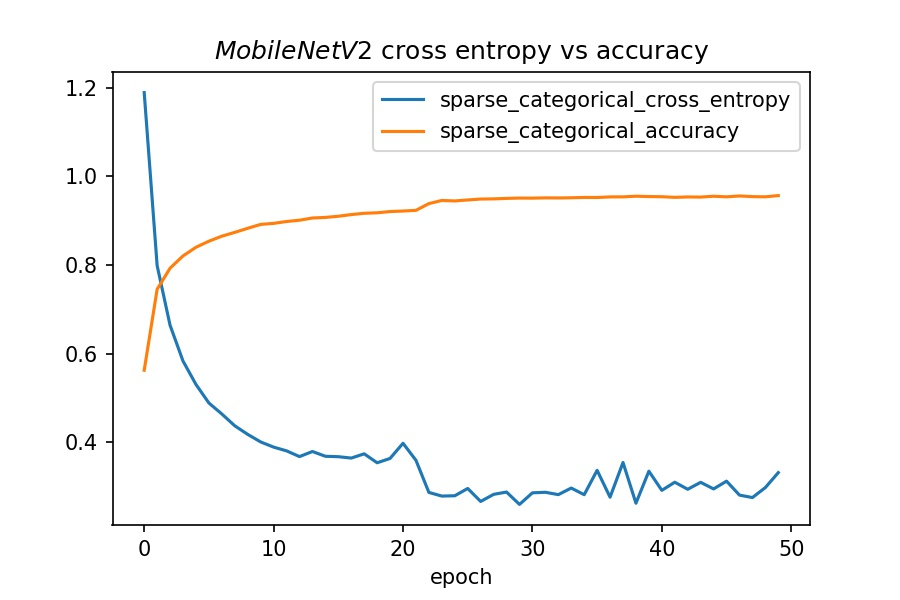
\includegraphics[width=\linewidth]{history_cross_entropy_accuracy.jpeg}
\caption{\texttt{MobileNetV2} training cross entropy vs accuracy}
\label{fig:mobilenetv2-2}
\end{figure}

\begin{figure}[h!]
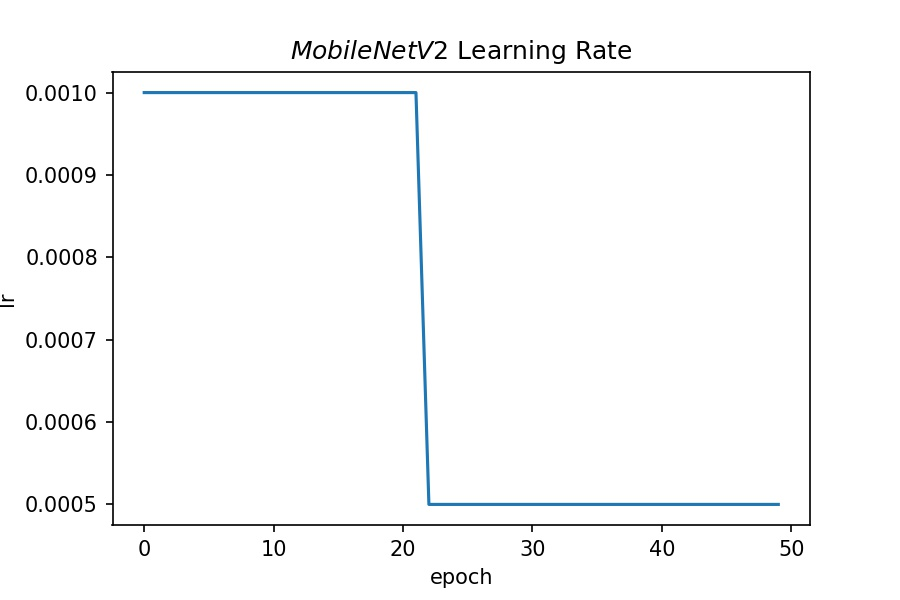
\includegraphics[width=\linewidth]{history_lr.jpeg}
\caption{\texttt{MobileNetV2} training learning rate}
\label{fig:mobilenetv2-3}
\end{figure}

\begin{figure}[h!]
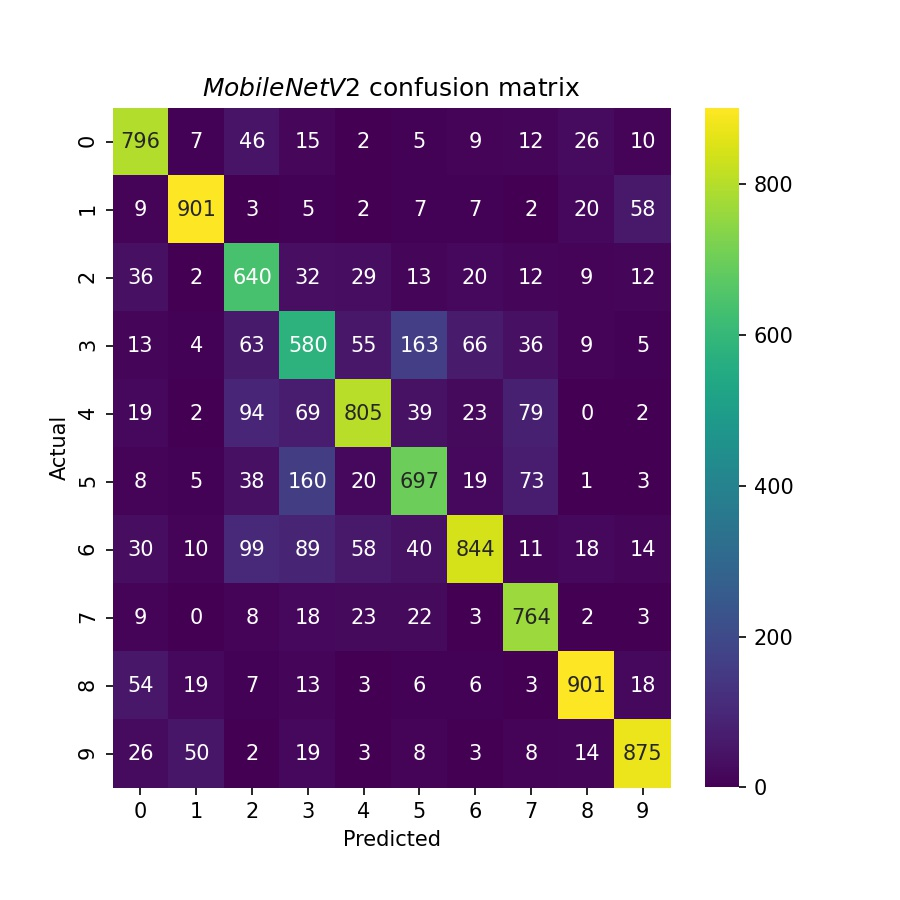
\includegraphics[width=\linewidth]{confusion_matrix.jpeg}
\caption{\texttt{MobileNetV2} confusion matrix}
\label{fig:mobilenetv2-4}
\end{figure}

\end{document}